
\documentclass[11pt]{article}

\marginparwidth 0.2in 
\oddsidemargin 0.1in 
\evensidemargin 0.1in 
\marginparsep 0.1in
\topmargin 0.1in 
\textwidth 6.5in \textheight 8 in

\usepackage[counterclockwise, figuresleft]{rotating}
\usepackage{hyperref}  
\usepackage{listings}
\usepackage{array}
\usepackage{tabularx}
\usepackage{attachfile}

\begin{document}

\author{İbrahim Burak Tanrıkulu, 21827852}
\title{BBM436 Microprocessors Lab.\\Assignment 6\\Asynchronous Serial Communication with Bit Banging}
\maketitle

\section{Introduction}
\begin{figure}[h!]
	\centering
	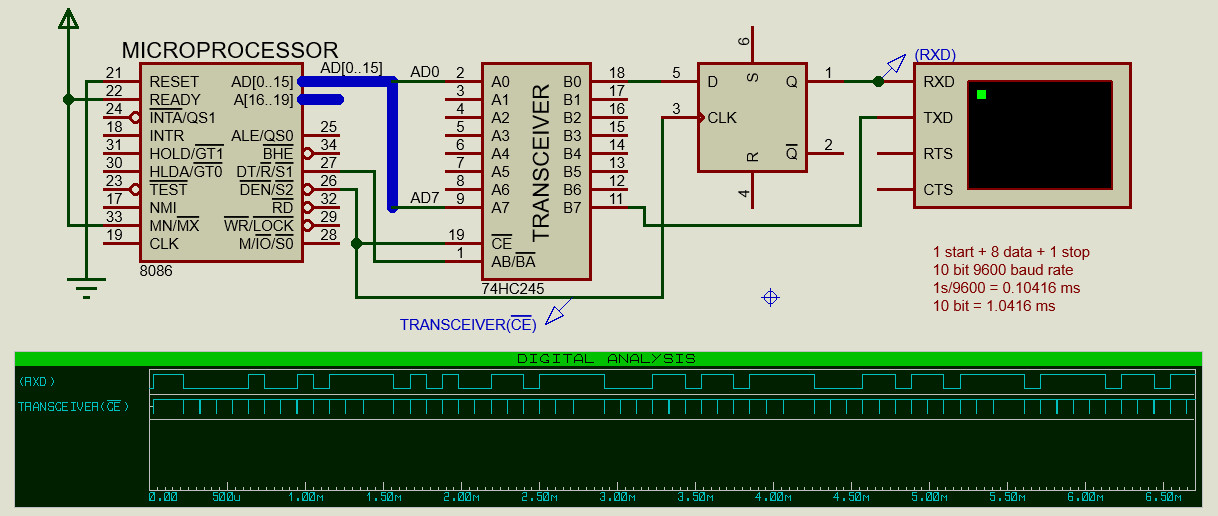
\includegraphics[width=17cm]{Tasarım.png}
	\caption{Design}
	\label{fig:Tasarım}
\end{figure}
Serial communication devices use 2 wire to communicate. RXD port for receive, TXD port for transmit data. In this assignment, i will use data 0 pin for TXD and data 7 port for RXD.
\\ In this assignment, we will use 1 start bit, 8 data bits and 1 stop bit. Also communication speed will be 9600 baud. So, we will use (1/9600)*10 seconds (1,0416 ms) for receiving or transmitting \\1 byte data. 
\\IN and OUT instructions uses address and data. Thus, i used Transceiver to pure data. But this Transceiver transmits a data for very short time. But we want to transmit bit for 0.10416 ms. \\So i added D flip-flop. D flip-flop takes data when Transceiver's Chip Enable signal's rising edge.
\section{Bit Banging}
In this phase, i printed "Hello" on virtual terminal with serial communication by bit banging. \\Firstly, i searched internet and found 8086 instructions' clock cycles. Then, i used simulation to get timings. After that, i calculated how many insruction we need for 0.1 ms and set this number to CX register. For delaying i used LOOP instruction. So i got same baud rate with virtual terminal. Then started to transmitting data. For data transmitting, i created a procedure and called whenever i wanted to print a character.
\\I used data port 0 to transmit bits. For transmitting 1 byte of data, we need 10 stage. First stage and last stage are start and stop bits. I did these stages by manually (setting AX to 00H or FFH). But at stage 1-9, its automated. I used rotate right(ROR) instruction for this purpose. Basically, transmit first bit of data, rotate right, so that second bit is now first bit. Loop it to transmit all.
\\If you wanted to print something else, you just change BL register with ASCII code of character and call "PRINTCHAR" procedure.
\begin{figure}[h!]
	\centering
	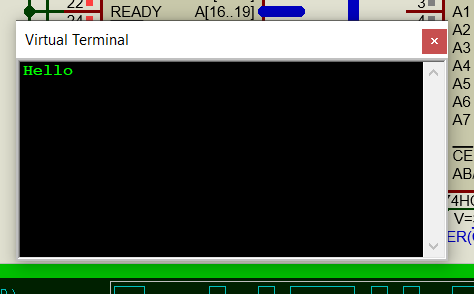
\includegraphics[width=10cm]{Terminal1.png}
	\caption{Design}
	\label{fig:Terminal output with bit banging}
\end{figure}
\section{Interrupt}
In this phase, whenever i enter a character to virtual terminal, terminal transmits this character to our microprocessor and microprocessor transmits this character back(echo).
\\When Phase 1 (transmitting hello) completes, an interrupt occurs. Before, I created an Interrupt Service Routine and moved his address to Interrupt Vector Table. So, when an interrupt occurs, this routine starts.
\\In this routine, i used data port 7 to receive data. Created a loop for IDLE stage (If input is 1, then continue, else break). When IDLE stage ends and start bit taken; microprocessor reads bits. 
\\I created an algorithm for that. Microprocessor reads bit from data port 7. Thus i used shift right (SHR) instruction and OR instruction.
\\Read data with IN instruction. Read data(AX register) is 80H or 00H. Our result register is BX.
\\ OR BX, AX -- inserting readed 8th bit to BX
\\ SHR BX, 1 -- shifting right for next concatenation.
\\ Loop 8 times.
\\ When we completed reading, we call PRINTCHAR procedure that i created in Phase 1 and transmit this character back to virtual terminal. Also i looped that interrupt too for infinitely echoing.
\begin{figure}[h!]
	\centering
	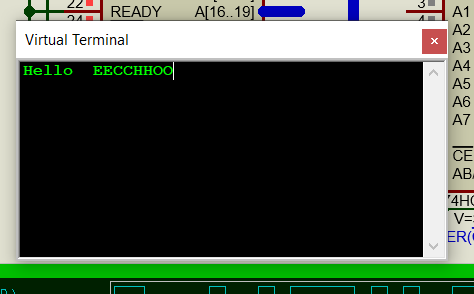
\includegraphics[width=10cm]{Terminal2.png}
	\caption{Design}
	\label{fig:Terminal echo with Interrupt}
\end{figure}
\\You can find the Project here: \attachfile{Assignment6.pdsprj}

\end{document}
